% Figura: fluxograma do OrderBased (versão consolidada)
\documentclass[tikz,border=4pt]{standalone}
\usepackage[utf8]{inputenc}
\usepackage[T1]{fontenc}
\usepackage{helvet}
\renewcommand{\familydefault}{\sfdefault}
\usepackage{amsmath}
\usepackage[eulergreek]{sansmath}
\sansmath
\usetikzlibrary{shapes.geometric,arrows.meta,positioning,fit,backgrounds,calc}
\tikzset{
  etapa/.style={draw=blue!60!black, rounded corners=4pt, fill=blue!4, inner sep=8pt},
  bloco/.style={draw=black!70, rounded corners=2pt, fill=white, align=center,
                font=\small, minimum height=1.1cm, text width=2.9cm},
  decisao/.style={diamond, draw=black!70, fill=yellow!15, aspect=1.8, align=center,
                  font=\small, inner sep=1pt},
  fim/.style={draw=black!70, rounded corners=8pt, fill=green!12, align=center,
              font=\small, minimum height=1.0cm, text width=3.1cm},
  falha/.style={draw=red!60!black, rounded corners=8pt, fill=red!8, align=center,
                font=\small, minimum height=0.8cm},
  seta/.style={-{Stealth[length=2.2mm]}, line width=0.7pt},
  rotetapa/.style={font=\small\bfseries, text=blue!60!black, anchor=south west},
}
\begin{document}
\hyphenpenalty=10000\exhyphenpenalty=10000
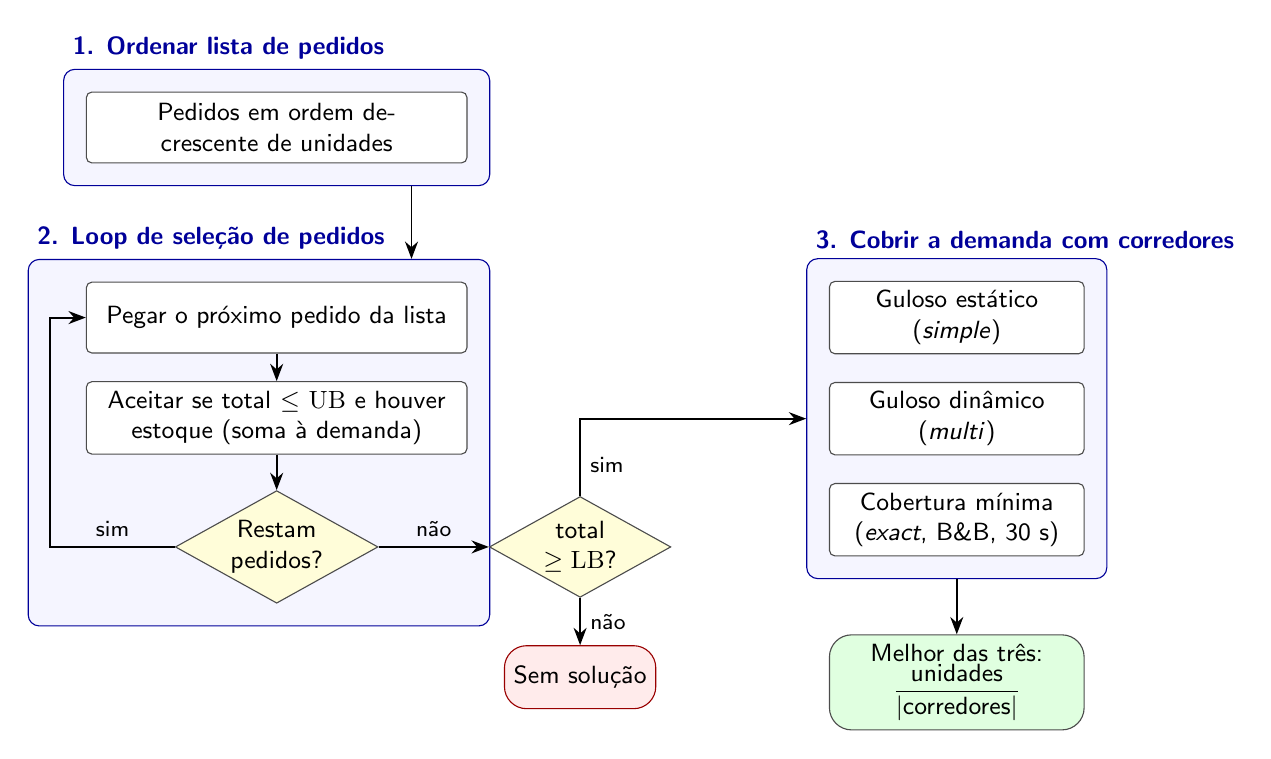
\begin{tikzpicture}[node distance=0.35cm]
\tikzset{pq/.style={bloco, minimum height=0.9cm}}

% ---------- 2. Loop de seleção de pedidos ----------
\node[pq, text width=4.6cm] (prox) {Pegar o próximo pedido da lista};
\node[pq, above=1.5cm of prox, text width=4.6cm] (ord) {Pedidos em ordem decrescente de unidades};
% ---------- 1. Ordenar lista de pedidos ----------

\begin{scope}[on background layer]
  \node[etapa, fit=(ord)] (e1) {};
\end{scope}
\node[rotetapa] at (e1.north west) {1. Ordenar lista de pedidos};

\node[pq, below=of prox, text width=4.6cm] (aceita) {Aceitar se $\text{total} \leq \mathrm{UB}$ e houver estoque (soma à demanda)};
\node[decisao, below=0.45cm of aceita] (resta) {Restam\\pedidos?};
\coordinate (lp) at ($(prox.west)+(-0.45,0)$);
\begin{scope}[on background layer]
  \node[etapa, fit=(prox)(aceita)(resta)(lp)] (e2) {};
\end{scope}
\node[rotetapa] at (e2.north west) {2. Loop de seleção de pedidos};
\draw[seta] ([xshift=-1.0cm]e1.south east) -- ([xshift=-1.0cm]e1.south east |- e2.north);
\draw[seta] (prox) -- (aceita);
\draw[seta] (aceita) -- (resta);
\draw[seta] (resta.west) -- node[above, font=\footnotesize] {sim} (resta.west -| lp) -- (lp) -- (prox.west);

% ---------- verificação de LB ----------
\node[decisao, right=1.4cm of resta] (lb) {$\text{total}$\\$\geq \mathrm{LB}$?};
\draw[seta] (resta.east) -- node[above, font=\footnotesize] {não} (lb.west);
\node[falha, below=0.6cm of lb] (nada) {Sem solução};
\draw[seta] (lb) -- node[right, font=\footnotesize] {não} (nada);

% ---------- 3. Cobrir a demanda com corredores ----------
\node[pq, right=2.0cm of lb.east |- prox, text width=3.0cm] (sim) {Guloso estático (\textit{simple})};
\node[pq, below=of sim, text width=3.0cm] (mul) {Guloso dinâmico (\textit{multi})};
\node[pq, below=of mul, text width=3.0cm] (exa) {Cobertura mínima (\textit{exact}, B\&B, 30 s)};
\begin{scope}[on background layer]
  \node[etapa, fit=(sim)(mul)(exa)] (e3) {};
\end{scope}
\node[rotetapa] at (e3.north west) {3. Cobrir a demanda com corredores};
\draw[seta] (lb.north) -- node[right, font=\footnotesize, pos=0.4] {sim} (lb.north |- e3.west) -- (e3.west);

\node[fim, below=0.7cm of e3, text width=3.0cm] (res) {Melhor das três:\\$\dfrac{\text{unidades}}{|\text{corredores}|}$};
\draw[seta] (e3) -- (res);

\end{tikzpicture}
\end{document}
